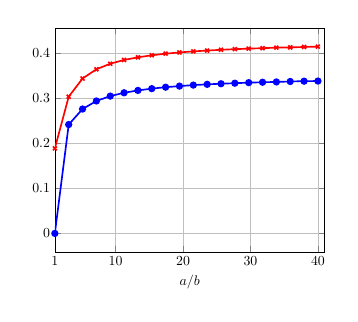
\begin{tikzpicture}[scale=0.5]
\begin{axis}[xlabel=$a/b$,ymajorgrids=true,xmajorgrids=true,xmin=1,xmax=41,xtick={1,10,20,30,40}]
%%%%%%%%%%% NATURAL CONFIGURATION
\addplot[Blue,mark=*,very thick] coordinates {(1.0,1.0000100001e-05) (3.05263157895,0.241770838761) (5.10526315789,0.276248551959) (7.15789473684,0.294120835945) (9.21052631579,0.304963575952) (11.2631578947,0.312330491726) (13.3157894737,0.317584754795) (15.3684210526,0.321510583527) (17.4210526316,0.324731668369) (19.4736842105,0.327161166349) (21.5263157895,0.329355925138) (23.5789473684,0.33105173157) (25.6315789474,0.332444903396) (27.6842105263,0.333598072823) (29.7368421053,0.334840190507) (31.7894736842,0.335700199107) (33.8421052632,0.336393890255) (35.8947368421,0.337413900455) (37.9473684211,0.338114433776) (40.0,0.338403384034) };
%%%%%%%%%%% MODIFIED CONFIGURATION
\addplot[Red,mark=x,very thick] coordinates {(1.0,0.188871888719) (3.05263157895,0.303648299641) (5.10526315789,0.343945018398) (7.15789473684,0.364483644836) (9.21052631579,0.376898505827) (11.2631578947,0.385203852039) (13.3157894737,0.391088647729) (15.3684210526,0.395587113766) (17.4210526316,0.399120306993) (19.4736842105,0.401940861514) (21.5263157895,0.404268253209) (23.5789473684,0.40603353402) (25.6315789474,0.407802499078) (27.6842105263,0.409176723346) (29.7368421053,0.410372524778) (31.7894736842,0.411359903073) (33.8421052632,0.412539388552) (35.8947368421,0.413152552578) (37.9473684211,0.414009929573) (40.0,0.414804148041) };
\end{axis}
\end{tikzpicture}
%%% Local Variables:
%%% mode: latex
%%% TeX-master: "../../mainManuscript"
%%% End:
